\section{Gaussian processes}


%%%%%%%%%%%%%%%%%%%%%%
\subsection{Introduction}
%%%%%%%%%%%%%%%%%%%%%%

\begin{frame}{What comes to $your$ mind when you hear ``Gaussian processes''?}
\end{frame}

\begin{frame}{Gaussian processes}
\begin{center}
	\only<1>{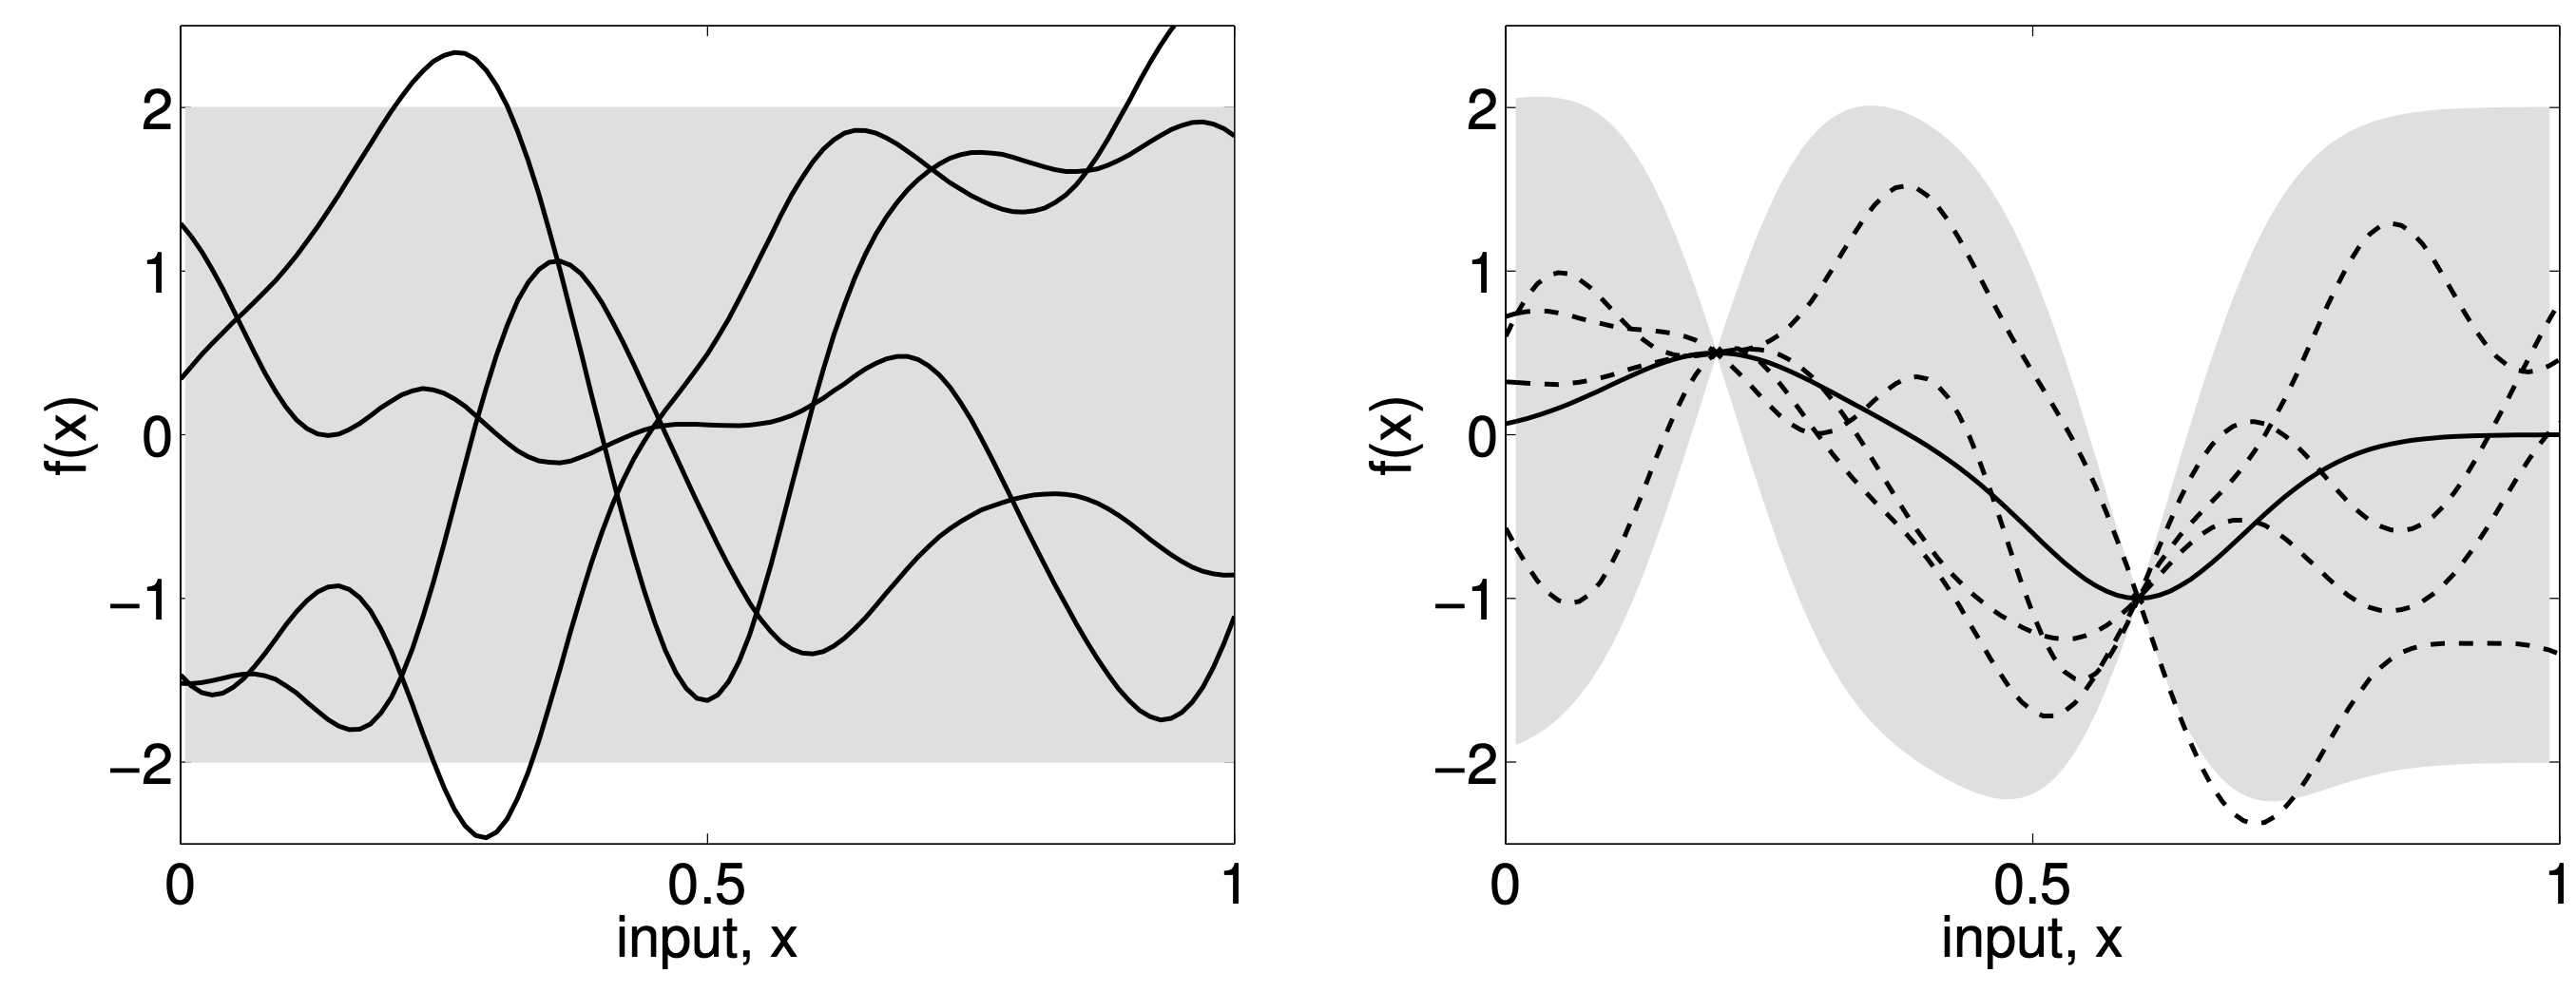
\includegraphics[height=.45\textheight]{figures_julyan/gp/gprw1}}
	\only<2>{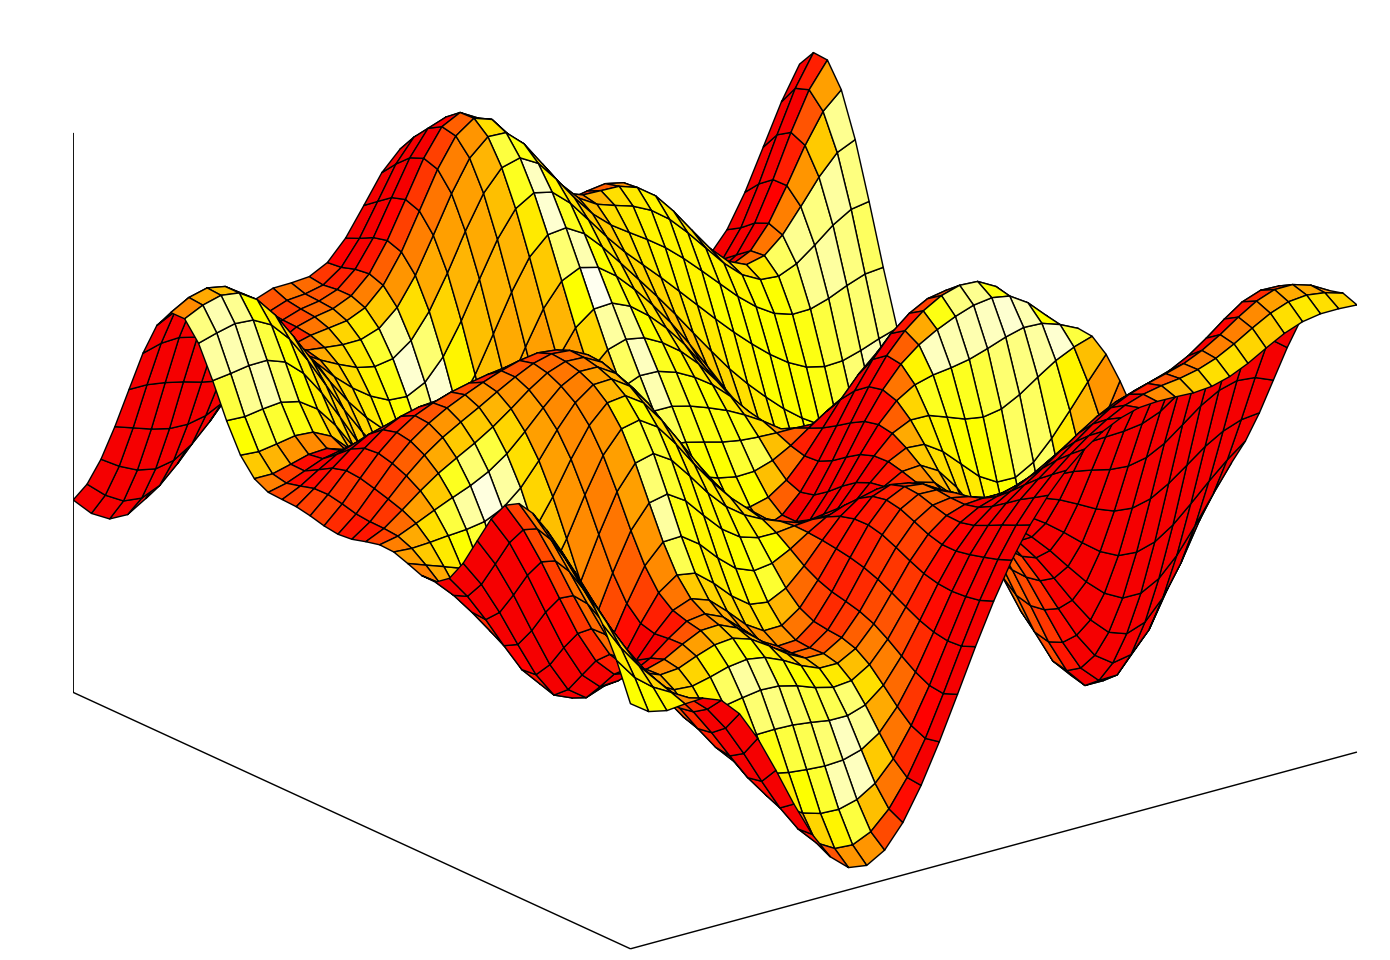
\includegraphics[height=.6\textheight]{figures_julyan/gp/gprw2}}
\end{center}
\hfill From \citet{Rasmussen:2006aa}
\end{frame}

\begin{frame}{Gaussian processes}
%\textcolor{gray}{What this chapter is about:}
%\begin{itemize}
%	\item How to use GPs in Bayesian inference
%	\item RKHS
%\end{itemize}\pause
%\textcolor{gray}{What this chapter is not about:}
%\begin{itemize}
%	\item Relationship with regularization theory, splines, support vector machines
%	\item PAC-Bayes analysis
%	\item Approximation methods: GP prediction methods is intractable for large sample $n$ datasets with complexity $\mathcal{O}(n^3)$ due to inversion of $n\times n$ matrix
%\end{itemize}\pause
\textcolor{gray}{Links with other chapters:}
\begin{itemize}
	\item GPs are used are BNP priors on curves
	\item As such, the properties of the induced posterior are studied in the section on asymptotics
	\item Wide limit in Bayesian neural networks
\end{itemize}
\end{frame}



\begin{frame}{References}
\begin{itemize}
	\item \alert{Main reference on GPs}: \fullcite{Rasmussen:2006aa}
	\item \alert{GPs in Bayesian inference}: Chapter 11 of \fullcite{ghosal2017fundamentals}
	\item \alert{Chapter 18} on Gaussian processes of \fullcite{murphy2023probabilisticMLadvanced}
\end{itemize}
\end{frame}




\begin{frame}{Supervized learning}

Two common approaches to \alert{supervized learning}:
\begin{itemize}
	\item restrict the class of functions considered, for example only linear functions of the input
	\item give a prior probability to every possible function, where higher probabilities are given to functions that we consider to be more likely
\end{itemize}

\end{frame}



\begin{frame}{Gaussian processes}
\begin{block}{Definition \citep{Rasmussen:2006aa}}
	A \alert{Gaussian process} is a collection of random variables, any finite number of which have a joint Gaussian distribution.
\end{block}

\pause

\begin{block}{Definition \citep{ghosal2017fundamentals}}
	A \alert{Gaussian process} is a stochastic process $W =(W_t: t \in T)$ indexed by an arbitrary set $T$ such that the vector $(W_{t_1},\ldots,W_{t_k})$ possesses a multivariate
normal distribution, for every $t_i\in T$ and $k\in \mathbb{N}$. A Gaussian process $W$ indexed by $\mathbb{R}^d$ is called:
\begin{itemize}
	\item  \alert{self-similar} of index $\alpha$ if $(W_{\sigma t}:t \in \mathbb{R}^d)$ is distributed like $(\sigma^\alpha W_{t}:t \in \mathbb{R}^d)$, for every $\sigma  > 0$, and 
	\item \alert{stationary} if $(W_{t+h}:t \in \mathbb{R}^d)$  has the same distribution of $(W_{t}:t \in \mathbb{R}^d)$, for every $h\in \mathbb{R}^d$.
\end{itemize}
\end{block}

\end{frame}



\begin{frame}{Mean function and covariance kernel}

Vectors $(W_{t_1},\ldots,W_{t_k})$ are called \alert{marginals}, and their distributions \alert{marginal distributions} or \alert{finite-dimensional distributions}

\pause


\begin{block}{Mean function and covariance kernel}
Finite-dimensional distributions are determined by the \alert{mean function} and \alert{covariance kernel}, defined by
$$\mu(t) = \mathbb{E}(W_t), \quad 
K(s, t) = \text{Cov}(W_s, W_t), \quad s, t \in  T.$$
\end{block}
\end{frame}



\begin{frame}{Scaling}

\begin{alertblock}{Scaling}
If $W =(W_t: t \in \mathbb{R}^d)$ is a Gaussian process  with covariance kernel $K$, then the process $(W_{\sigma t}: t \in \mathbb{R}^d)$ is another Gaussian process, with covariance kernel $K(\sigma s, \sigma t)$, for any $\sigma  > 0$. A scaling factor $\sigma  > 1$ shrinks the sample paths, whereas a factor $\sigma  < 1$ stretches them.
\end{alertblock}

\pause

\begin{center}
	\only<2>{
	$\sigma  > 1$ \hspace{4.5cm} $\sigma  < 1$ 
	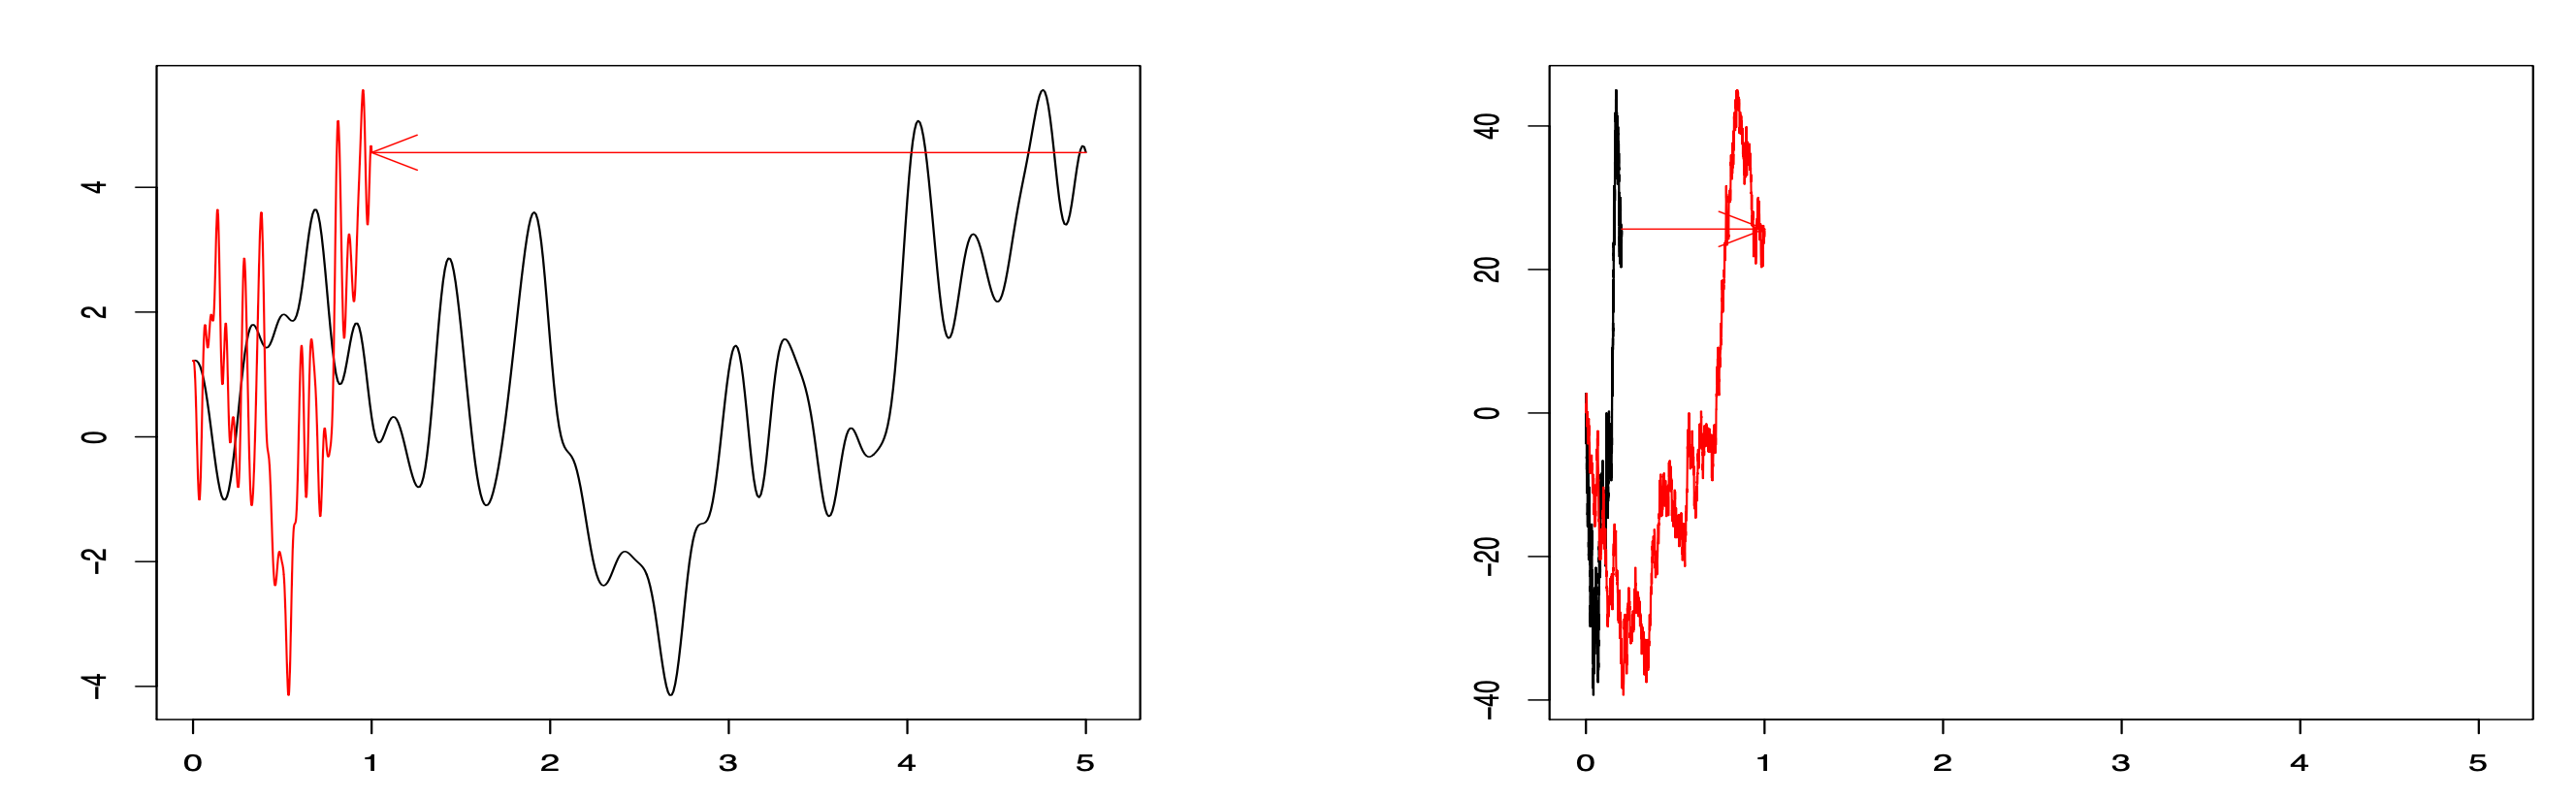
\includegraphics[height=.35\textheight]{figures_julyan/gp/scaling}
	}
\end{center}
\hfill From \citet{ghosal2017fundamentals}


\end{frame}


\subsection{Examples}


\begin{frame}{Examples}
\begin{exampleblock}{Random series}
	If $Z_1,\ldots,Z_m\simiid \mathcal{N}(0,1)$ and $a_1,\ldots,a_m$ are [deterministic] functions, then the \textit{Random series} $W_t = \sum_{i=1}^m a_i(t)Z_i$ defines a Gaussian process with:\bigskip
	
		\indent $\mu(t)=$\bigskip
		
		\indent $K(s, t)=$
%	\begin{align*}
%		\mu(t) & = \\
%		K(s, t) & = 
%	\end{align*}
\end{exampleblock}

\end{frame}


\begin{frame}{Examples}

\begin{exampleblock}{Brownian motion (or Wiener process)}
	The \textit{Brownian motion} is the zero-mean Gaussian process, say on $[0,\infty)$, with continuous sample paths and covariance function $K(s,t)=\min(s,t)$.
\end{exampleblock}

\pause


\begin{alertblock}{Brownian motion properties}
	Let $B_t$ be a Brownian motion, then $\forall s< t$:
	\begin{itemize}
		\item \alert{Stationarity}:  $B_t-B_s\sim \mathcal{N}(0,t-s)$
		\item \alert{Independent increments}:  $B_t-B_s\ind (B_u, u\leq s)$
	\end{itemize}
	Thus it is a L\'evy process.
	\begin{itemize}
		\item \alert{Self-similar} of index $1/2$.
	\end{itemize}
\end{alertblock}

\end{frame}


\begin{frame}{Examples}

\begin{exampleblock}{Ornstein--Uhlenbeck}
	The standard \textit{Ornstein--Uhlenbeck process} with parameter $\theta>0$ is a mean-zero, stationary GP with time set $T = [0, \infty)$, continuous sample paths, and covariance function
		$$K(s,t) = (2\theta)^{-1}\exp\left(-\theta|t-s|\right).$$
\end{exampleblock}

\pause

\begin{alertblock}{Properties of Ornstein--Uhlenbeck process}
	The standard Ornstein--Uhlenbeck process with parameter $\theta>0$ can be constructed from a Brownian motion $B$ through the relation 	
	$$W_t = (2\theta)^{-1/2}\exp\left(-\theta t\right)B_{e^{2\theta t}}.$$
\end{alertblock}

\pause

Relationship between [fixed learning rate] \alert{stochastic gradient descent} (SGD) and \alert{Markov chain Monte Carlo} (MCMC) through the Ornstein--Uhlenbeck process: see \citet{mandt2017stochastic}.


\end{frame}


\begin{frame}{Examples}

	
\begin{exampleblock}{Square exponential}
	GP with covariance function (a.k.a. radial basis function kernel)
	$$K(s,t) = \exp\left(-\frac{\Vert t-s\Vert^2}{2\ell^2}\right).$$
	Parameter $\ell$ is called the \textit{characteristic length-scale}.
\end{exampleblock}


\begin{exampleblock}{Fractional Brownian motion}
	The \textit{fractional Brownian motion} (fBm) with \textit{Hurst parameter} $\alpha\in  (0, 1)$ is the mean zero Gaussian process $ W = (W_t : t \in  [0, 1])$ with continuous sample paths and covariance function
	$$K(s,t) = \frac{1}{2}\left(s^{2\alpha}+t^{2\alpha}-|t-s|^{2\alpha}\right).$$
	\begin{itemize}
		\item $\alpha=2$ yields the standard Brownian motion.
	\end{itemize}
\end{exampleblock}
	
\end{frame}



\begin{frame}{Kriging}

\begin{exampleblock}{Kriging}
	For a given Gaussian process $W = (W_t : t \in T)$ and fixed, distinct points $t_1,\ldots,t_m \in T$, the conditional expectations $W_t^\star  = \mathbb{E}[ W_t|W_{t_1},\ldots,W_{t_m}]$ define another Gaussian process.
\end{exampleblock}

\pause 

\begin{block}{Exercise}
	Find the covariance function of $W_t^\star$, say $K^\star(t,s)$, as a function of $(t_1,\ldots,t_m)$.
\end{block}

\pause 

\begin{alertblock}{Properties of Kriging}
	\begin{itemize}
		\item If $W$ has continuous sample paths, then so does $W^\star$. 
		\item In that case the process $W^\star$ converges to $W$ when $m \to \infty$  and the interpolating points $(t_1,\ldots,t_m)$ grow dense in $T$.
	\end{itemize}
\end{alertblock}
\end{frame}

\subsection{Reproducing kernel Hilbert space}

\begin{frame}{Reproducing kernel Hilbert space}
	To every Gaussian process corresponds a Hilbert space, determined by its covariance kernel. This space determines the support and shape of the process, and therefore is crucial for the properties of the Gaussian process as a prior. 

\pause

\begin{block}{Definition}
	A \textit{Hilbert space} is an inner product space that is complete wrt the distance function induced by the inner product.
\end{block}
\end{frame}


\begin{frame}{Reproducing kernel Hilbert space}
For a Gaussian process $W = (W_t : t \in T)$, let $\overline{\text{lin}}(W)$ be the closure of the set of all linear combinations $\sum_I \alpha_i W_{t_i}$ in the $L_2$-space of square-integrable variables. The space $\overline{\text{lin}}(W)$ is a Hilbert space.

\pause

\begin{block}{Definition} 
The \textit{reproducing kernel Hilbert space} (RKHS) of the mean-zero, Gaussian process $W = (W_t : t \in T )$ is the set $\mathbb{H}$ of all functions $z_H:T \to \mathbb{R}$ defined by $z_H(t) = \mathbb{E}(W_t H)$, for $H$ ranging over $\overline{\text{lin}}(W)$. The corresponding inner product is
	$$\langle z_{H_1},z_{H_2}\rangle_{\mathbb{H}} =  \mathbb{E}(H_1H_2).$$
\end{block}
\end{frame}


\begin{frame}[allowframebreaks]{Reproducing kernel Hilbert space}

\begin{alertblock}{Properties of RKHS}
	\begin{itemize}
		\item Correspondance $z_H \leftrightarrow H$ is an isometry (by def of inner product), so the definition is well-posed (the correspondence is one-to-one), and $H$ is indeed a Hilbert space.
		\item Function corresponding to $H=\sum_I \alpha_i W_{s_i}$ is \bigskip
			$z_H=$
		\item For any $s\in T$, function $K(s,\cdot)$ is in RKHS $\mathbb{H}$ associated with $H = W_s$.
	\end{itemize}
\end{alertblock}

\framebreak

\begin{alertblock}{Reproducing formula}
For a general function $z_H \in \mathbb{H}$ we have $$\langle z_H, K(s, \cdot)\rangle_{\mathbb{H}} = \mathbb{E}(H W_s) = z_H(s).$$
That is to say, for any function  $h \in \mathbb{H}$,
	$$h(t) = \langle h, K(t, \cdot)\rangle_{\mathbb{H}}.$$
\end{alertblock}

\end{frame}

\begin{frame}{Example of RKHS: Euclidean space}
%	\begin{exampleblock}{Euclidean space}
%		
%	\end{exampleblock}
%	\vfill 
\end{frame}

